\chapter{Failure, Distributed Consensus}
\section{Failure}
A dependable system must satisfy four properties: \begin{itemize}
\item \textbf{Availability}: The system is ready to be used immediately at any point in time.
\item \textbf{Reliability}: The system can run continuously without failure.
\item \textbf{Safety}: If the system (temporarily) fails to operate correctly, nothing catastrophic will happen.
\item \textbf{Maintainability}: The system can be repaired relatively easily.
\end{itemize}
Building a dependable system comes down to controlling failure and faults. 

First, it is important to define what failure \textit{is}: \begin{itemize}
\item \textbf{Failure}: a system fails when it fails to meet its promises or cannot provide its services in the specified manner
\item \textbf{Error}: part of the system state that leads to failure (i.e., it differs from its intended value)
\item \textbf{Fault}: the cause of an error (results from design errors, manufacturing faults, deterioration, or external disturbance)
\end{itemize}
Note that a failure can be recursive: \begin{itemize}
\item Failure may be initiated by a mechanical fault 
\item Manufacturing fault leads to disk failure 
\item Disk failure is a fault that leads to database failure 
\item Database failure is a fault that leads to email service failure 
\end{itemize}

In a \textit{total failure}, all components in a system fail; this is typical for a non-distributed system. In a \textit{partial failure}, one or more (but not all) components in a distributed system fail - that is, some components are affected, but other components are completely unaffected; this is treated as a fault for the whole system.

\subsection{Classifications}
Distributed systems are designed at the process level, so we consider failures that are visible at the process level first.

\subsubsection{Crash Failure}
A process undergoes crash failure when it permanently ceases to execute its actions. This is an irreversible change.

In an asynchronous model, crash failures cannot be detected with total certainty, since there is no lower bound of the speed at which a process can execute its actions. 

In a synchronous system where processor speed and channel delays are bounded, crash failures can be detected using timeouts. 

\subsubsection{Omission Failure}

If the receiver does not receive one or more of the messages sent by the transmitter, an omission failure occurs. For wireless networks, this can occur when a collision occurs in the MAC layer or when a receiving node moves out of range.

\subsubsection{Transient Failure}

A transient failure can disturb the state of processes in an arbitrary way. The agent inducing this problem may be momentarily active but it can have a lasting effect on the global state. Examples include a power surge, mechanical shock, or lightning.

\subsubsection{Byzantine Failure}

Byzantine failures represent the weakest of all of the failure models. It allows every conceivable form of erroneous behaviour. The term alludes to uncertainty and was first proposed by Pease et al.

Assume that process $i$ forwards the value $x$ of a local variable to each of its neighbours. The following inconsistencies may occur: \begin{itemize}
\item two distinct neighbours $j$ and $k$ receive values $x$ and $y$, where $x \neq y$.
\item one or more neighbours do not receive any data from $i$.
\item every neighbour receives a value $z$ where $z \neq x$.
\end{itemize}

Possible causes of Byzantine failures include:
\begin{itemize}
\item total or partial breakdown of a link joining $i$ with one of its neighbours.
\item software problems in process $i$.
\item hardware synchronization problems – assume that every neighbour is connected to the same bus, and is attempting to read the same copy sent out by $i$. However, since the clocks are not perfectly synchronized, they may attempt to read the value of $x$ at the same local time but at different absolute times. If the value of $x$ varies with time, then each neighbour of $i$ may read different values of $x$. 
\end{itemize}

\subsubsection{Software Failure}
Software failure is failure originating from within the software. Note that many of the other types of failure, such as crash, omission, transient and Byzantine failures, originate from software issues. For example, a poorly designed loop that does not terminate can appear as a crash failure to external observers. Similarly, an inadequate policy in routing software can cause packets to drop, resulting in omission failure.

Causes of software failure include: \begin{itemize}
\item \textbf{Coding or human error}: As an example, the program may have used the wrong physical parameters. On September 23, 1999, NASA lost the Mars Climate Orbiter spacecraft (valued at 327.6 million USD) to this class of error; one team used metric units while another team used imperial units, resulting in the spacecraft entering the Mars atmosphere at a much lower altitude than expected and promptly disintegrating. This trajectory discrepancy is illustrated in \autoref{fig:marsclimateorbiter-mishapdiagram}. 
\item \textbf{Software design error}: The software was designed in such a way that errors can arise in its functionality. The Mars Pathfinder mission landed without issues on the Martian surface on July 4, 1997. However, its ability to communicate failed due to a design flaw in the real-time embedded software kernel VxWorks; this flaw was later determined to have originated from a priority inversion scenario: \begin{itemize}
\item A low priority task $\mathtt{LP}$ locks file $\mathtt{F}$.
\item A high priority task $\mathtt{HP}$ is scheduled next, which also needs to lock file $\mathtt{F}$.
\item A medium priority $\mathtt{MP}$ task (with high CPU requirement) becomes ready to run.
\item $\mathtt{MP}$ is the highest priority unblocked task; as a result, it is allowed to run, and consumes all CPU.
\item $\mathtt{LP}$ has no CPU available to it and thus idles indefinitely. However, even though $\mathtt{HP}$ is higher priority than $\mathtt{MP}$, $\mathtt{MP}$ is still being run, and $\mathtt{HP}$ cannot be scheduled as $\mathtt{LP}$ still has the lock on $\mathtt{F}$. As a result, \textit{priority inversion} occurs: $\mathtt{HP}$ is indirectly prevented from running by $\mathtt{MP}$.
\end{itemize}
\item \textbf{Memory leaks}: Processes fail to fully free up the physical memory that has been allocated to them. This effectively reduces the size of available physical memory over time. When the available memory falls below the minimum requirement by the system, a crash becomes inevitable.
\item \textbf{Inadequacy of specification}: An issue with the specification may have long-lasting ramifications that are only apparent when the bounds of the specification are exceeded. The canonical example is the Y2K problem, in which years in dates were only stored with two digits; this became problematic with the turn of the century where the "year" would roll over from $99$ to $00$.
\end{itemize}

\begin{figure}
\centering
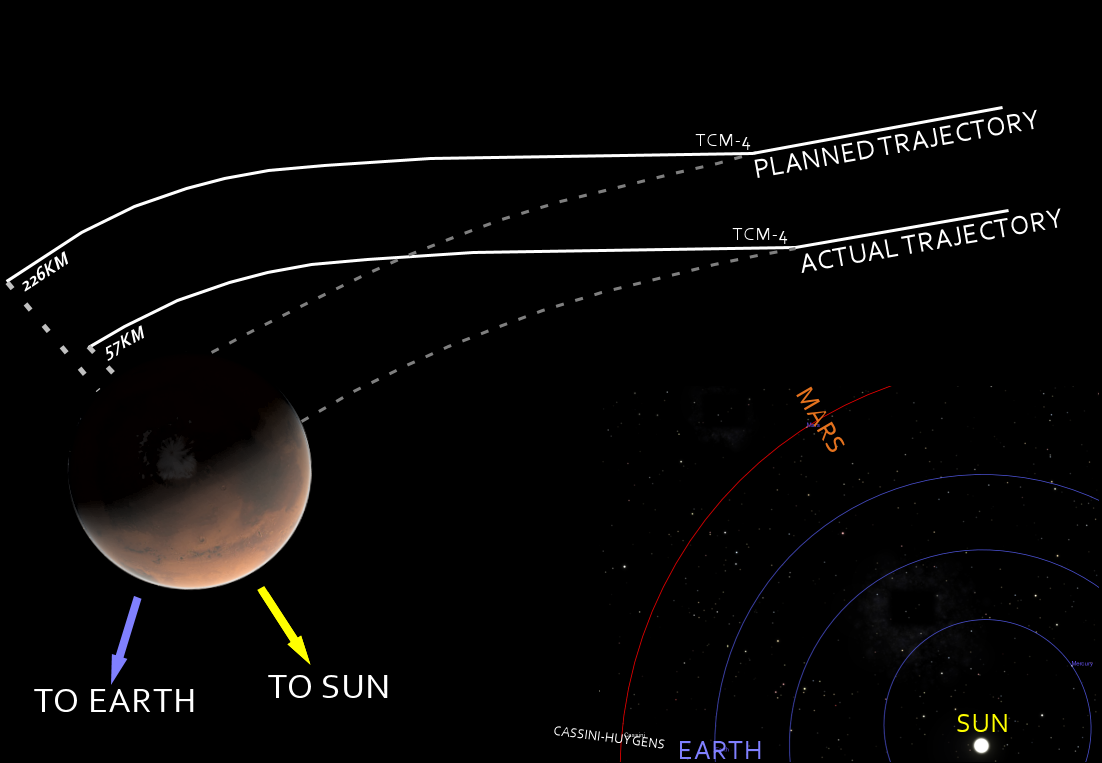
\includegraphics[width=0.7\linewidth]{figures/Mars_Climate_Orbiter_-_mishap_diagram}
\caption[Mars Climate Orbiter wrong trajectory]{The incorrect trajectory calculated for the Mars Climate Orbiter. Courtesy of \href{https://en.wikipedia.org/wiki/Mars_Climate_Orbiter\#/media/File:Mars_Climate_Orbiter_-_mishap_diagram.png}{Wikipedia}.}
\label{fig:marsclimateorbiter-mishapdiagram}
\end{figure}

\subsubsection{Temporal Failure}
Real-time systems require actions to be completed within a specific time frame. When this time limit is not met, a temporal failure occurs.

\subsubsection{Security Failure}
Viruses and other malicious software may lead to unexpected behaviour, which may manifest as a system fault. 

\subsubsection{Human Error}
Human errors can also play a large part in system failure. Examples include: \begin{itemize}
\item In November 1988, a significant portion of the long distance service along the East Coast of the United States of America was disrupted when a construction crew accidentally detached a major fibre optic cable in New Jersey. As a result, 3,500,000 call attempts were blocked. 
\item On September 17, 1991 AT\&T technicians in New York failed to respond to an activated alarm for six hours as they were attending a seminar on warning systems. The resulting power failure blocked nearly 5 million domestic and international calls and paralysed air travel throughout the Northeast, causing nearly 1,170 flights to be cancelled or delayed. 
\end{itemize}

\subsection{Fault-Tolerant Systems}
We designate a system that does not tolerate failures as a fault-tolerant system. In such systems, the occurrence of a fault violates \textit{liveness} and \textit{safety} properties. Safety properties specify that "something bad never happens"; doing nothing easily fulfils a safety property as this will never lead to a "bad" situation. Safety properties are complemented by liveness properties, which assert that "something good" will eventually happen.

The first known fault-tolerant computer was SAPO, built in 1951 in Czechoslovakia by Antonin Svoboda. Most of the development in Long Life, No Maintenance (LLNM) computing was undertaken by NASA during the 1960s in preparation for Project Apollo and other research prospects. NASA's first machine went into a space observatory, and their second attempt, the JSTAR computer, was used in Voyager. This computer had a backup of memory arrays to facilitate the use of memory recovery methods; this led to the name of the JPL Self-Testing-And-Repairing computer. It could detect its own errors and fix them or bring up redundant modules as needed.

\subsubsection{Masking Tolerance}
Let $P$ be the set of configurations for the fault-tolerant system. Given a set of fault actions $F$, the fault span $Q$ corresponds to the largest set of configurations that the system can support. In a failure-masking system, when a fault $F$ is masked, its occurrence has no impact on the application (i.e. $P = Q$). 

Masking tolerance is important in many safety-critical applications where the failure can endanger human life or cause massive loss of properties; an aircraft must be able to fly even if one of its engines malfunctions. Masking tolerance preserve both safety and liveness properties of the original system. 

To implement failure masking, redundancy must be introduced. This includes information redundancy, time redundancy, and physical redundancy. This is illustrated in \autoref{fig:screenshot050}.
\begin{figure}
\centering
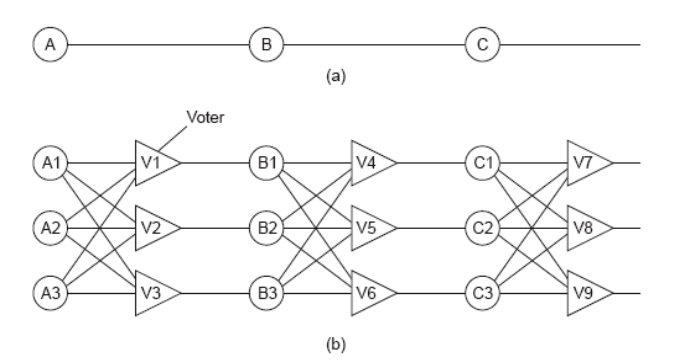
\includegraphics[width=0.7\linewidth]{figures/screenshot050}
\caption{Failure masking comparison.}
\label{fig:screenshot050}
\end{figure}

\subsection{Non-Masking Tolerance}
In non-masking fault tolerance, faults may temporarily affect and violate the safety property (i.e. $P \subset Q$). However, liveness is not compromised, and eventually normal behaviour is restored. As an example, consider watching a movie where the backend server crashes; the system can automatically restore the service by switching to a standby proxy server. 

Checkpointing and stabilisation represent two opposing scenarios in non-masking tolerance.  \begin{itemize}
\item \textit{Checkpointing} relies on history; recovery is achieved by retrieving lost computation.
\item \textit{Stabilisation} is history-insensitive and does not care about lost computation as long as eventual recovery is guaranteed. 
\end{itemize}

\subsection{Fail-Safe Tolerance}
Certain faulty configurations do not affect the application in an adverse way and are therefore considered harmless.  A fail-safe system relaxes the tolerance requirement by aiming to avoid the subset of faulty configurations that will have catastrophic consequences (not withstanding the failure), and allowing the remaining faulty configurations to occur.

As an example, at a four-way traffic crossing, collision is possible if the lights are green in both directions. However, if the lights are red, traffic may stall but there will be no catastrophic side effects.

\subsection{Graceful Degradation}
There are systems that neither mask nor fully recover from the effect of failures, but exhibit a degraded behaviour that falls short of normal behaviour, but is still considered acceptable.  The notion of acceptability is highly subjective and entirely dependent on the user running the application.

Examples include: \begin{itemize}
\item While routing a message between two points in a network, a program computes the shortest path. In the presence of a failure, the program returning a valid path that is not the shortest possible may be considered acceptable.
\item An operating system may switch to a safe mode where users cannot create or modify files, but can read the files that already exist.  
\end{itemize}

\section{Distributed Consensus}
Distributed consensus - that is, consensus amongst a distributed system - is a necessary requirement for many scenarios; it is easier to achieve in the absence of failures. Some of these scenarios are explored below: \begin{enumerate}
\item The leader election problem in a network of processes. Each process begins with an initial proposal for leadership. At the end, one of the candidates is elected as a leader; every process must agree on this.
\item Fund transfer
\item Clock synchronisation 
\end{enumerate}

The distributed consensus problem is formulated as such: a distributed system contains $n$ processes, and each process has an initial value in a mutually agreed domain. The challenge is to design a failure-resilient algorithm that allows processes to reach an irrevocable decision that fulfills the following conditions: \begin{itemize}
\item \textbf{Termination}: Every (non-faulty) process must eventually come to a decision.
\item \textbf{Agreement}: The final decision of every (non-faulty) process must be identical.
\item \textbf{Validity}: If every (non-faulty) process begins with the same initial value $v$, their final decision must be $v$. 
\end{itemize}

If there is no failure, then reaching an agreement is trivial. Reaching consensus, however, becomes surprisingly difficult when one or more members fail to execute actions. In the formulation of the problem, we assume that at most $k$ members ($k>0$) can fail; an important finding by Fischer et al. is that in a fully asynchronous system, it is impossible to reach consensus even if $k=1$. 

In discussion of distributed consensus, it is important to discuss \textit{bivalence} and \textit{univalence}. A decision state is bivalent if there exist at least two distinct executions leading to two distinct decision values (e.g. 0 or 1). On the other hand, a state from which only one decision value can be reached is called a univalent state. Univalent state states can be either 0-valent or 1-valent.

Consider a best-of-five-sets tennis match between A and B. If the score is 6-3, 6-4 in favour of A, the decision state is bivalent, since anyone can win at this point. However, if the score becomes 6-3, 6-4, 7-6 in favour of A, then the state becomes univalent. 

\subsection{The Byzantine Generals' Problem}
The Byzantine Generals' Problem, as described by \href{https://en.wikipedia.org/wiki/Byzantine_fault_tolerance\#Byzantine_Generals\%27_Problem}{Wikipedia}:
\begin{quotation}
[...] a group of generals, each commanding a portion of the Byzantine army, encircle a city. These generals wish to formulate a plan for attacking the city. In its simplest form, the generals must decide only whether to attack or retreat. Some generals may prefer to attack, while others prefer to retreat. The important thing is that every general agree on a common decision, for a halfhearted attack by a few generals would become a rout, and would be worse than either a coordinated attack or a coordinated retreat.


The problem is complicated by the presence of treacherous generals who may not only cast a vote for a suboptimal strategy, they may do so selectively. For instance, if nine generals are voting, four of whom support attacking while four others are in favor of retreat, the ninth general may send a vote of retreat to those generals in favor of retreat, and a vote of attack to the rest. Those who received a retreat vote from the ninth general will retreat, while the rest will attack (which may not go well for the attackers). The problem is complicated further by the generals being physically separated and having to send their votes via messengers who may fail to deliver votes or may forge false votes. 
\end{quotation}

Leslie Lamport showed by proof that for a system of $n + 1$ nodes, there cannot be more than $\frac{n}{3}$ faulty nodes if distributed consensus is desired. This can be reformulated in the terms of the Byzantine Generals' Problem: there must be more than $3m$ troops in an army with up to $m$ traitors to launch a concerted attack.
